\chapter{Анализ математической модели}
\label{ch:chap2}

\section{Анализ матриц}
Найдем собственные числа и собственные вектора матрицы $A$ модели (\ref{1_model_lin}).

\begin{equation}
    \begin{cases}
        \lambda_1 = 0 & v_1 = \begin{bmatrix}
            1 & 0 & 0 & 0
        \end{bmatrix}^T\\
         \lambda_2 = 0&  v_2 = \begin{bmatrix}
            -1 & 0 & 0 & 0
        \end{bmatrix}^T\\
         \lambda_3 = 2.4165 & v_3 = \begin{bmatrix}
            0.0165 & 0.0400 & 0.3820 & 0.9231
        \end{bmatrix}^T\\
         \lambda_4 = -2.4165 & v_4 = \begin{bmatrix}
            -0.0165 & 0.0400 & -0.3820 & 0.9231
        \end{bmatrix}^T
    \end{cases}
\end{equation}

Заметим, что в спектр матрицы $A$ входит число с положительной вещественной частью, следовательно, система $\ref{1_model_full}$ неустойчива.

Обратим внимание на то, что собственные векторы, соответствующие $\lambda_{1,2}=0$, являются линейно зависимыми. Они соответствуют только смещению координаты тележки без влияния на остальные переменные (то есть положение тележки не влияет на скорость тележки, угол отклонения маятника и угловую скорость маятника). Два других собственных вектора (соответствуют $\lambda_{3,4}$) указывают на то, что изменения линейной скорости тележки, угла отклонения маятника и угловой скорости маятника влияют друг на друга.

\subsection{Управляемость и стабилизируемость системы}
Составим матрицу управляемости и определим ее ранг

\begin{multline}
    U = \begin{bmatrix}
        B & AB & A^2B&A^3B
    \end{bmatrix} = \begin{bmatrix}
        0 &   0.0037  &       0  &  0.0005\\
    0.0037      &   0   & 0.0005   &      0\\
         0   & 0.0022   &      0  &  0.0127\\
    0.0022     &    0 &   0.0127   &      0
    \end{bmatrix} \Rightarrow\\
    \Rightarrow rank(U) = 4
\end{multline}
Ранг матрицы управляемости равен размерности системы, следовательно, система является полностью управляемой, а значит и стабилизируемой.


\subsection{Наблюдаемость и обнаруживаемость системы}

Составим матрицу наблюдаемости и определим ее ранг

\begin{equation}
    V = \begin{bmatrix}
        C \\ CA \\ CA^2\\ CA^3
    \end{bmatrix} = \begin{bmatrix}
           1&         0     &    0    &     0\\
         0   &      0 &   1  &      0\\
         0 &   1 &         0 &        0\\
         0     &    0&         0 &   1\\
         0    &     0 &    0.2529     &    0\\
         0     &    0 &   5.8395    &     0\\
         0     &    0    &     0  &  0.2529\\
         0     &    0    &     0   & 5.8395
    \end{bmatrix} 
    \Rightarrow rank(V) = 4
\end{equation}
Ранг матрицы наблюдаемости равен размерности системы, следовательно, система является полностью наблюдаемой, а значит и обнаруживаемой.

\section{Передаточные матрицы}

Найдем передаточную матрицу $W_{u \to y}(s)$

\begin{equation}
    W_{u \to y} (s) = C \left(sI-A  \right)^{-1}B = \begin{bmatrix}
        \frac{0.003747s^2 -0.02133}{s^4-5.839s^2}\\[2ex]
        \frac{0.002174}{s^2-5.839}
    \end{bmatrix}
\end{equation}

Динамический порядок $ \frac{0.003747s^2 -0.02133}{s^4-5.839s^2}$ равен 4, относительный динамический порядок 2; динамический порядок $\frac{0.002174}{s^2-5.839}$ равен 2, относительный динамический порядок равен 2.

Нули функции $\frac{0.003747s^2 -0.02133}{s^4-5.839s^2}$ равны $s_0 =\pm 2.3859$, полюса $s_p = \{ 0; 0; \pm 2.4165 \}$.

Полюса $\frac{0.002174}{s^2-5.839}$ равны $s_p = \{ \pm 2.4165 \}$.

Найдем передаточную матрицу $W_{f \to y}(s)$

\begin{equation}
    W_{f \to y} (s) = C \left(sI-A  \right)^{-1}D = \begin{bmatrix}
        \frac{0.002174}{s^2-5.839}\\[2ex]
        \frac{0.0502}{s^2-5.839}
    \end{bmatrix}
\end{equation}

Динамический порядок $ \frac{0.002174}{s^2-5.839}$ равен 2, относительный динамический порядок 2; динамический порядок $\frac{0.0502}{s^2-5.839}$ равен 2, относительный динамический порядок равен 2.

Полюса для  $ \frac{0.002174}{s^2-5.839}$ и $\frac{0.0502}{s^2-5.839}$ одинаковы и равны $s_p = \{ \pm 2.4165 \}$.

Заметим, что полюса всех передаточных функций содержат в себе собственные числа матрицы $A$ $\lambda_{3,4}$ -- для функций, кроме первой, полюса первой передаточной функции совпадают с собственными числами матрицы $A$.

С физической точки зрения, все передаточные функции описывают расходящийся переходный процесс при $u=0$ и $f=0$.


\section{Моделирование}

Зададим начальные условия $$x_{0_1} = \begin{bmatrix}
     0.01\\
    0.01\\
    0.01\\
    0.05
\end{bmatrix},  x_{0_2} = \begin{bmatrix}
    0.01\\
    0.01\\
    0.05\\
    0.01
\end{bmatrix},  x_{0_3} = \begin{bmatrix}
    0.01\\
    0.05\\
    0.01\\
    0.01
\end{bmatrix}$$
и выполним моделирование линеаризованного (\ref{1_model_lin}) и нелинеаризованного объекта (\ref{1_model_full}) на малом и большем отрезке времени: 1 и 10 секунд, соответственно.


\begin{figure}[!h]
\center{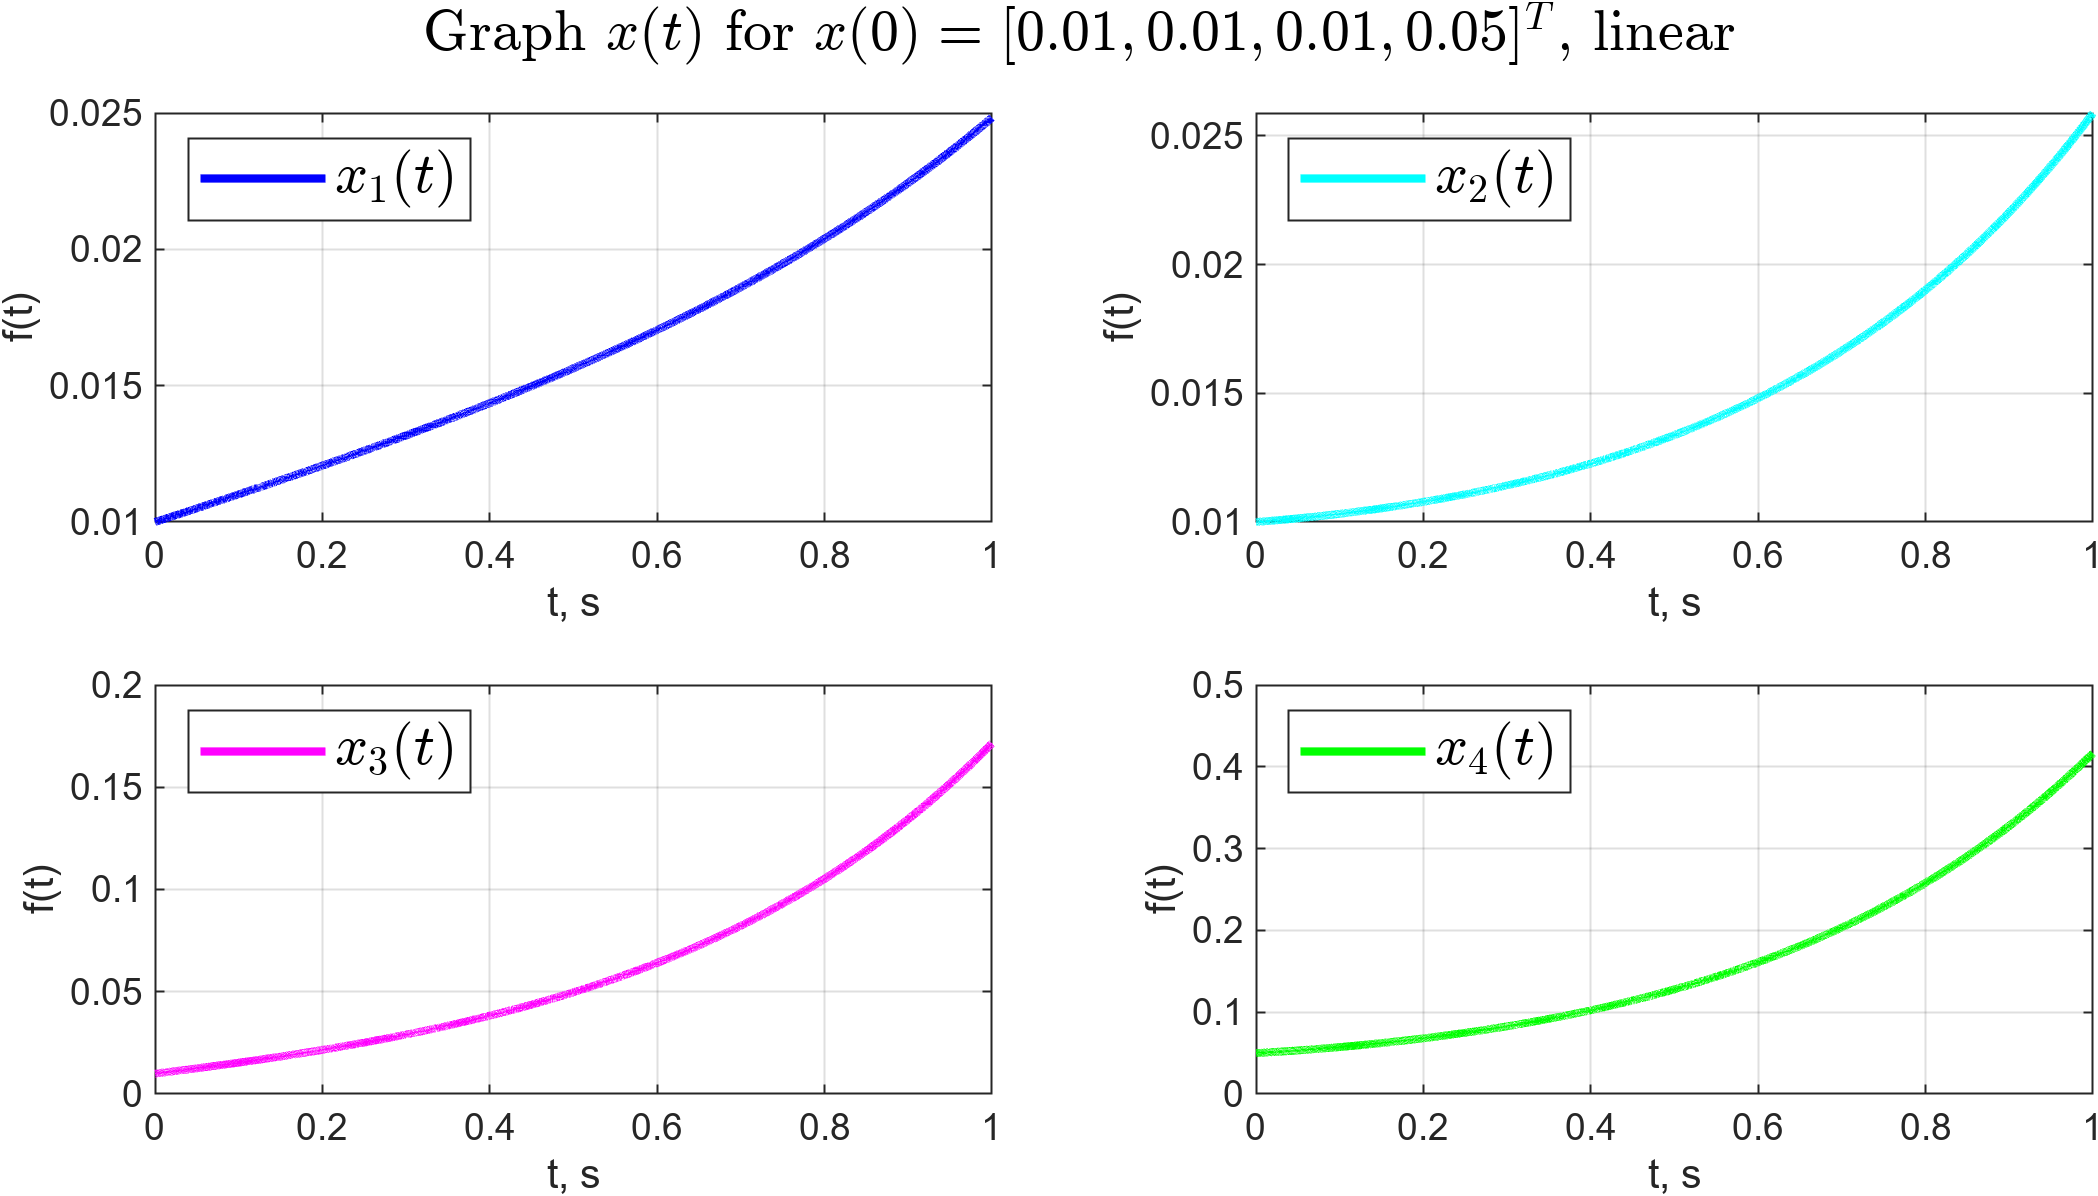
\includegraphics[width=1\linewidth]{pic/2_x_lin_04_sm.png}}
\caption{График вектора состояния линеаризованной системы, время моделирования $t=1$ с, начальные условия $x_{0_1}$.}
\label{2_x_lin_01_sm}
\end{figure}

\begin{figure}[!h]
\center{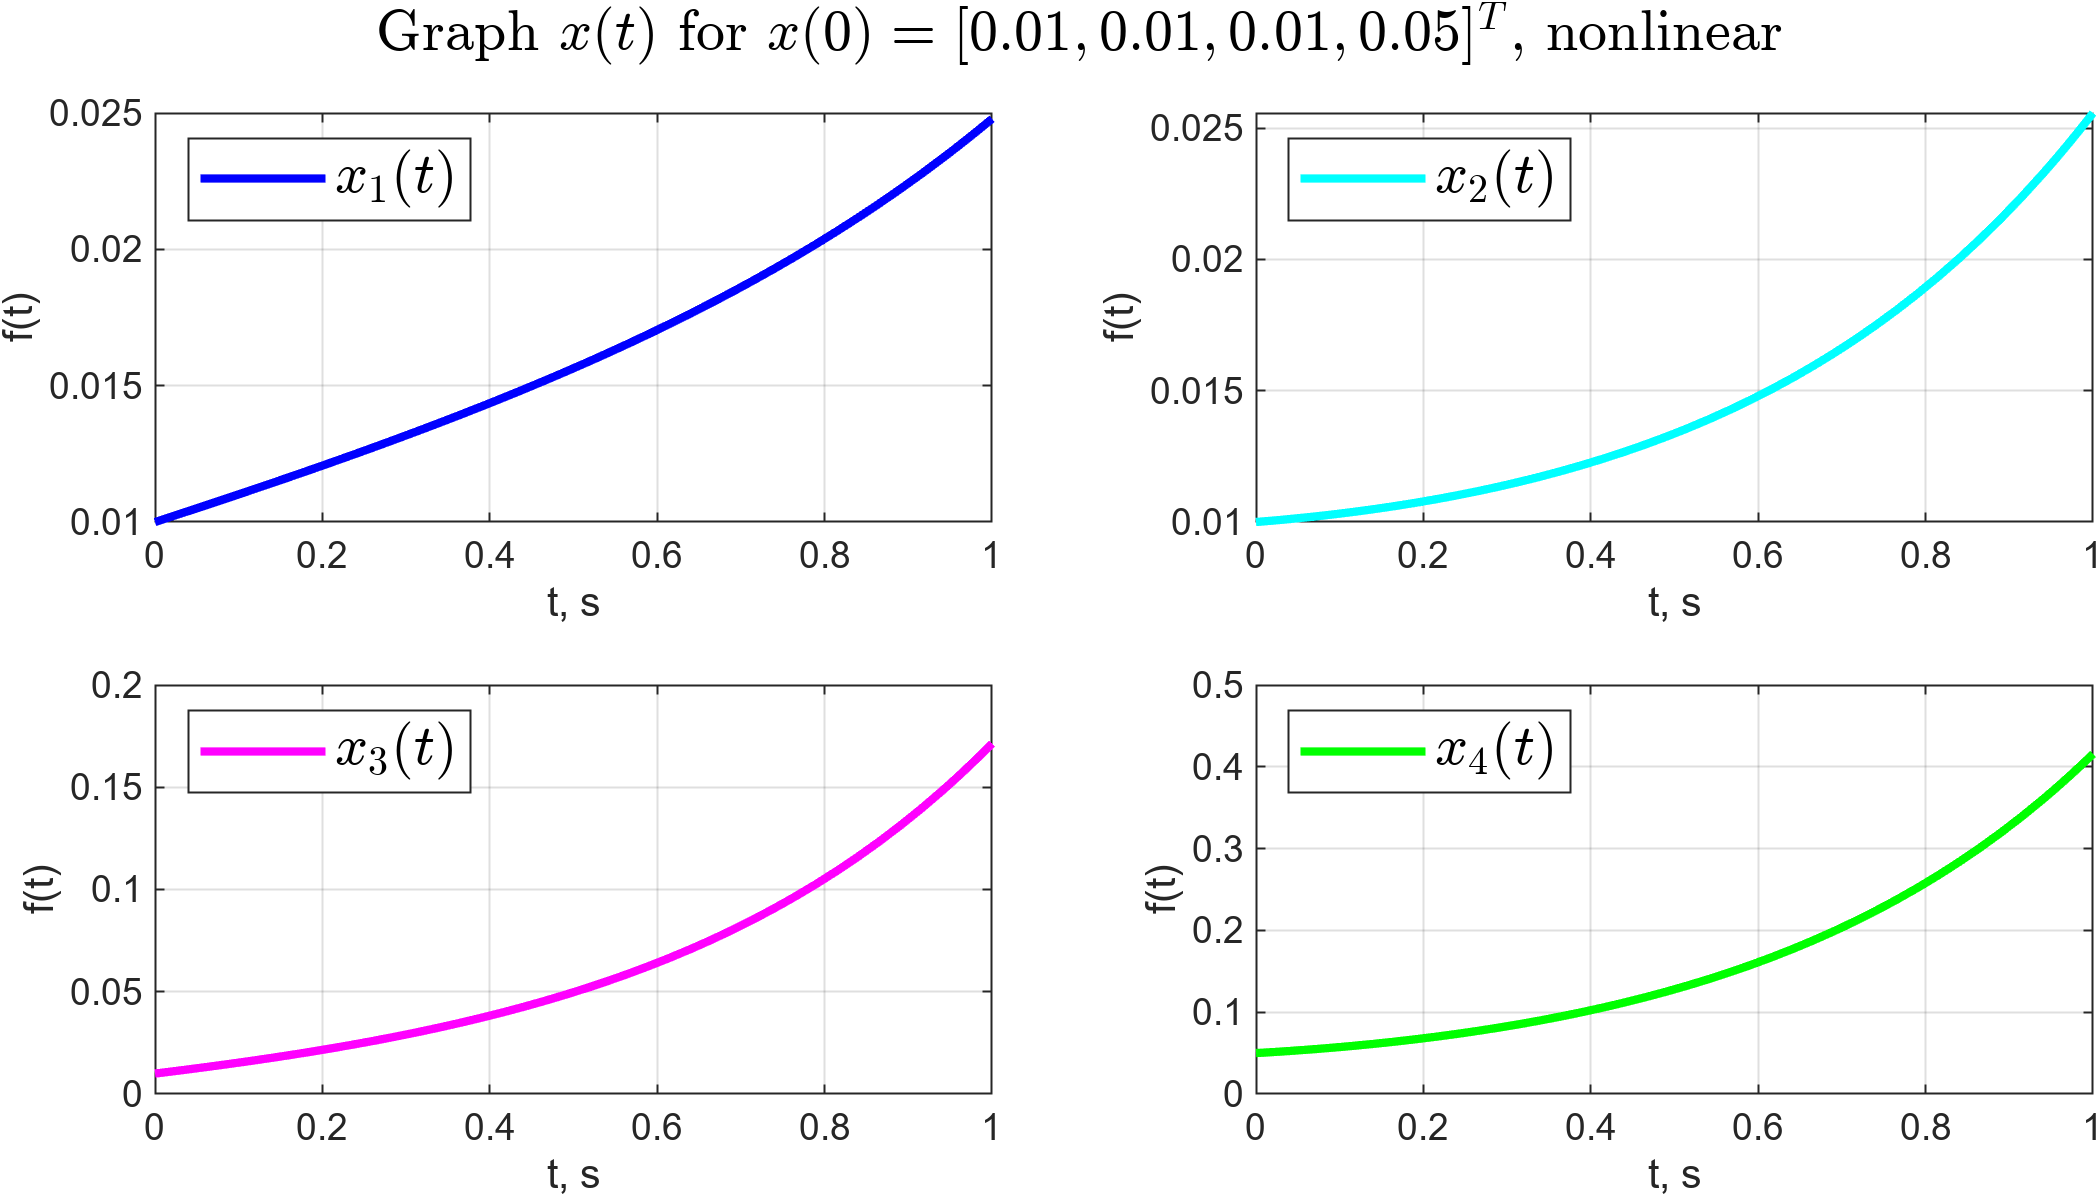
\includegraphics[width=1\linewidth]{pic/2_x_nlin_04_sm.png}}
\caption{График вектора состояния исходной системы, время моделирования $t=1$ с, начальные условия $x_{0_1}$.}
\label{2_x_nlin_01_sm}
\end{figure}

\begin{figure}[!h]
\center{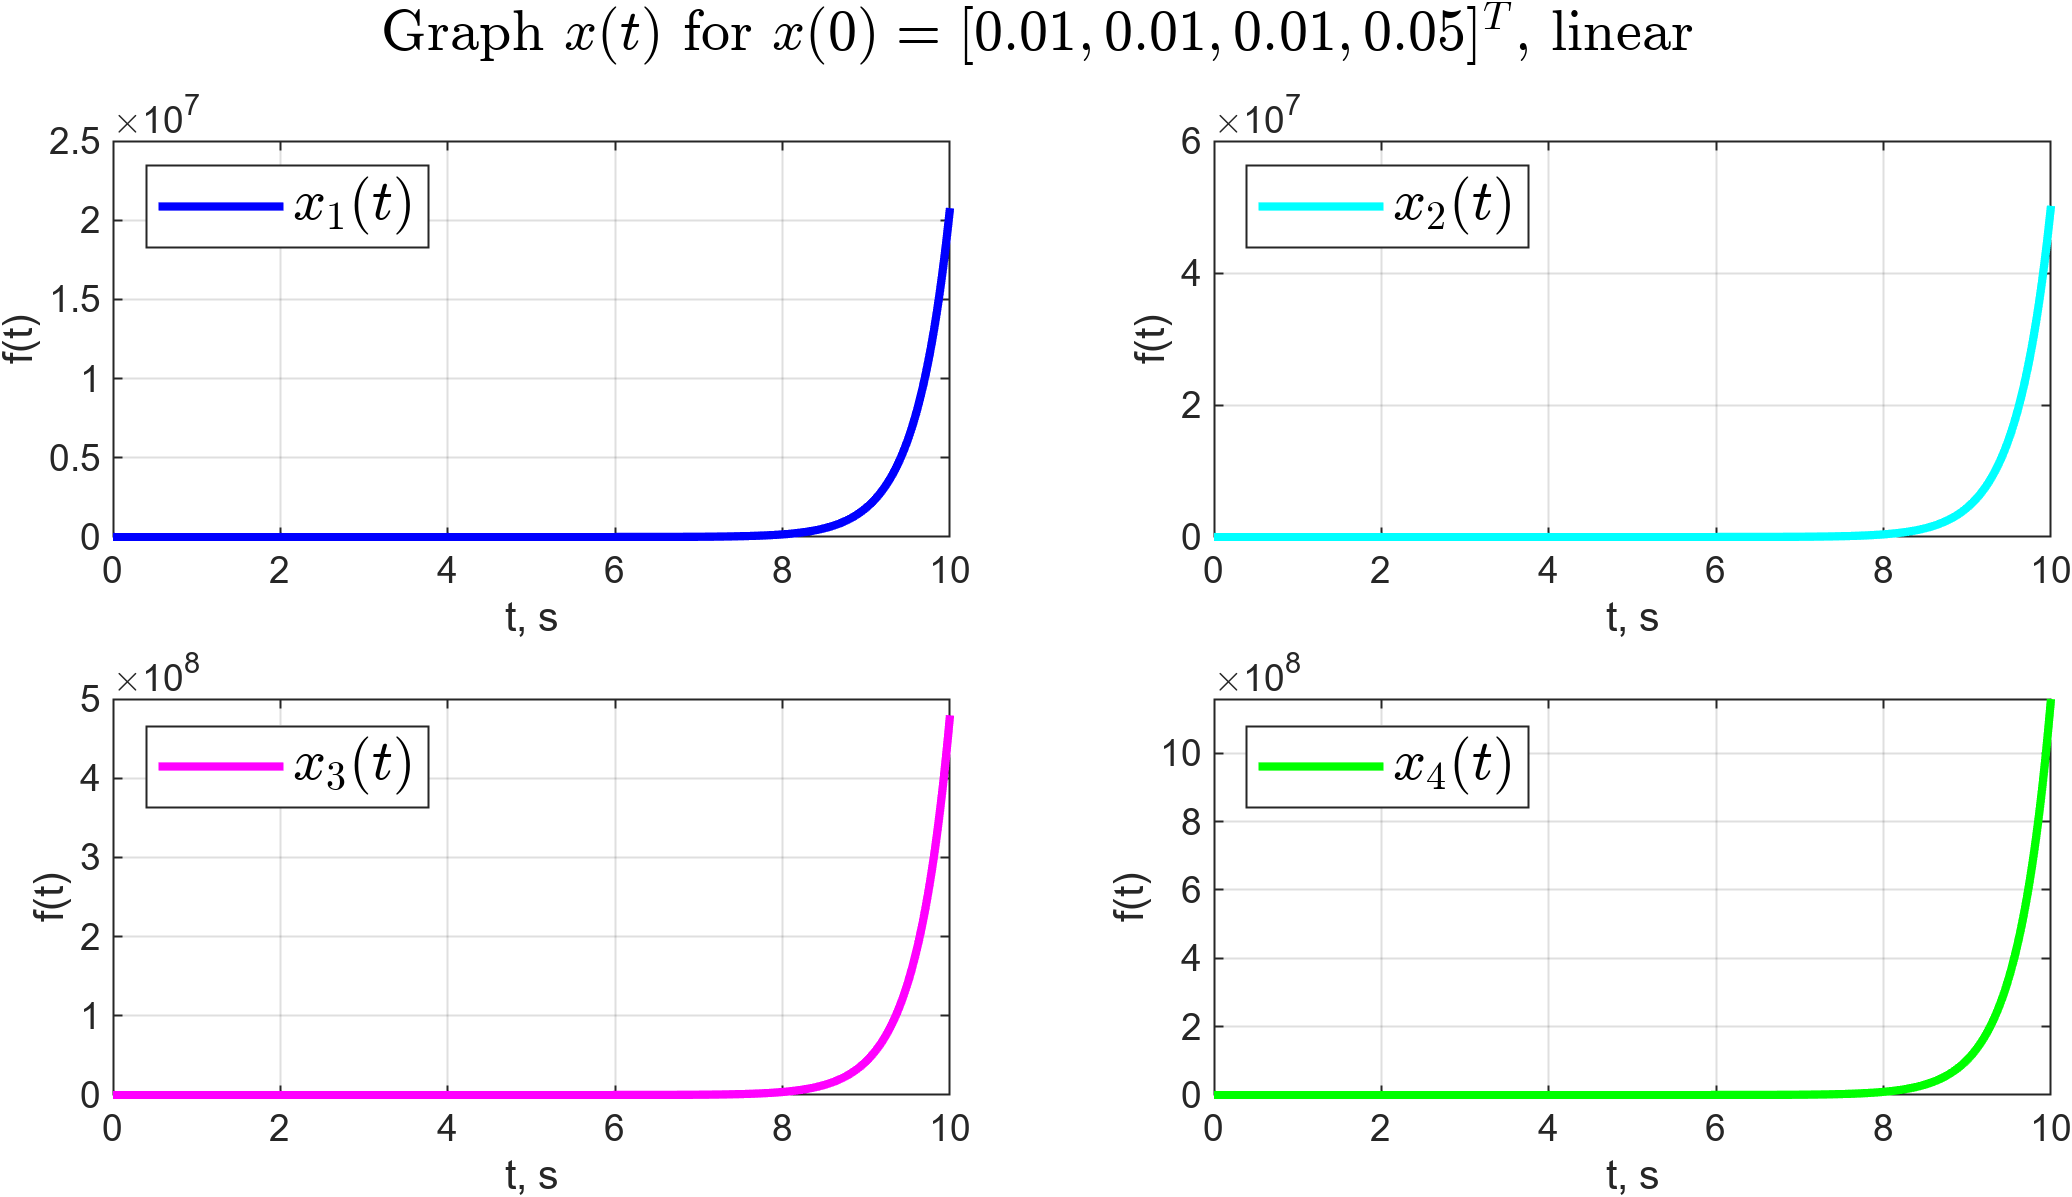
\includegraphics[width=1\linewidth]{pic/2_x_lin_04_lg.png}}
\caption{График вектора состояния линеаризованной системы, время моделирования $t=10$ с, начальные условия $x_{0_1}$.}
\label{2_x_lin_01_lg}
\end{figure}

\begin{figure}[!h]
\center{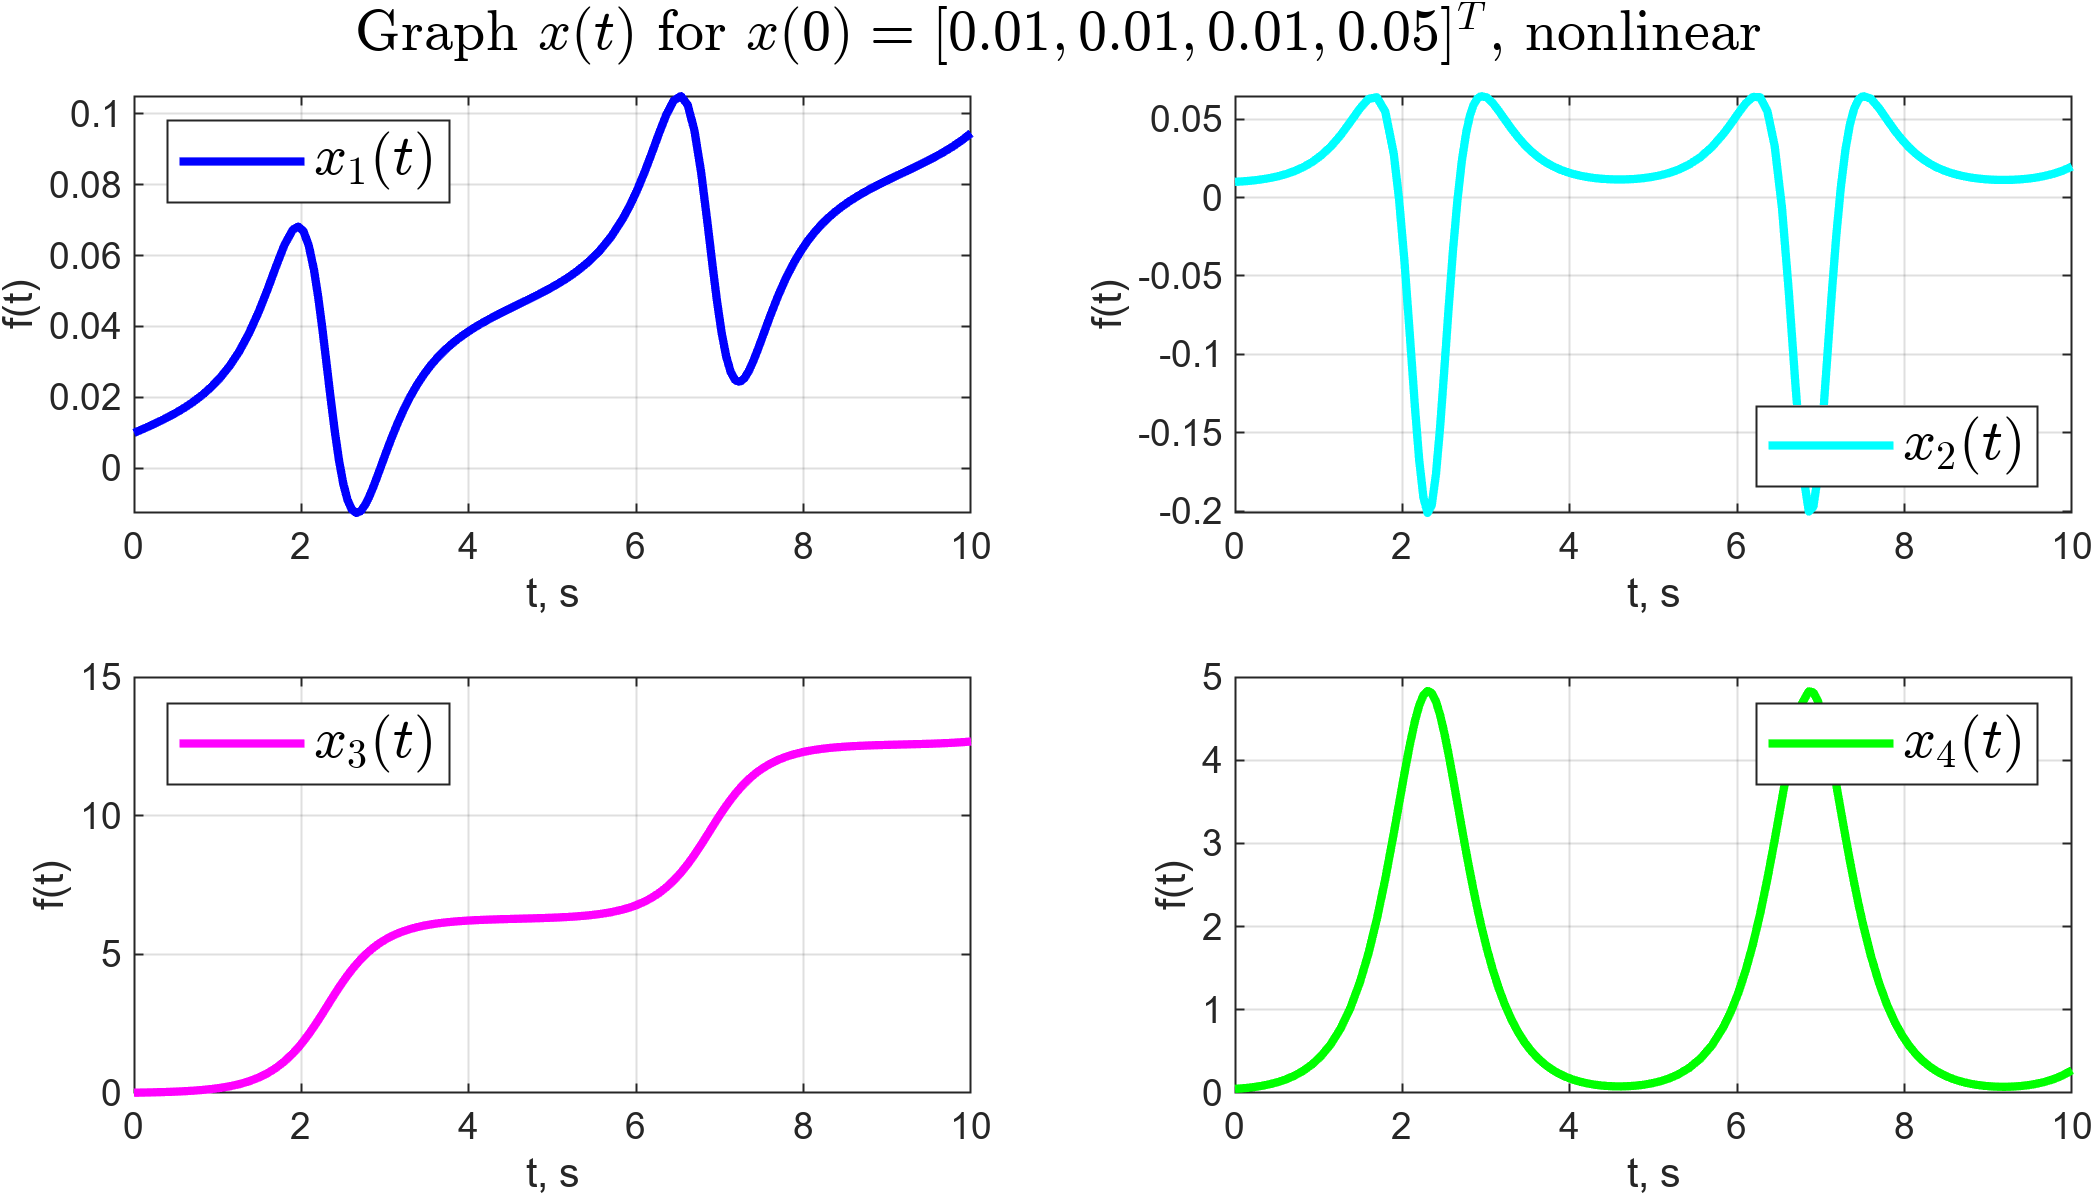
\includegraphics[width=1\linewidth]{pic/2_x_nlin_04_lg.png}}
\caption{График вектора состояния исходной системы, время моделирования $t=10$ с, начальные условия $x_{0_1}$.}
\label{2_x_nlin_01_lg}
\end{figure}

Заметим, что для малого времени моделирования ($t=1$ с) графики состояния линеаризованной и нелинеаризованной систем близки между собой, однако в случае увеличения времени моделирования до $t=10$ с, поведение линеаризованной модели сильно отличается от исходной. Это происходит потому, что в ходе линеаризации мы считали углы отклонения маятника от вертикали малыми. 

Поведение, которое мы наблюдаем для нелинеаризованной модели (рисунок \ref{2_x_nlin_01_lg}) близко к поведению реального физического объекта: координата тележки $x_1$ совершает колебания (то есть движется из стороны в сторону) с постепенным смещением вверх, график угла отклонения $x_3$ совершает переходы от $\pi k$ к $\pi(k+1), k \in \mathbf{Z}$ (то есть совершает обороты около точки крепления), кроме того, мы видим, что энергия системы сохраняется: максимальная по модулю угловая скорость маятника достигается в нижней точке, минимальная -- в верхней.


Далее выполним моделирование систем с начальными условиями $x_{0_2}$, то есть зададим  большее значение угла отклонения маятника от вертикали.
\begin{figure}[!h]
\center{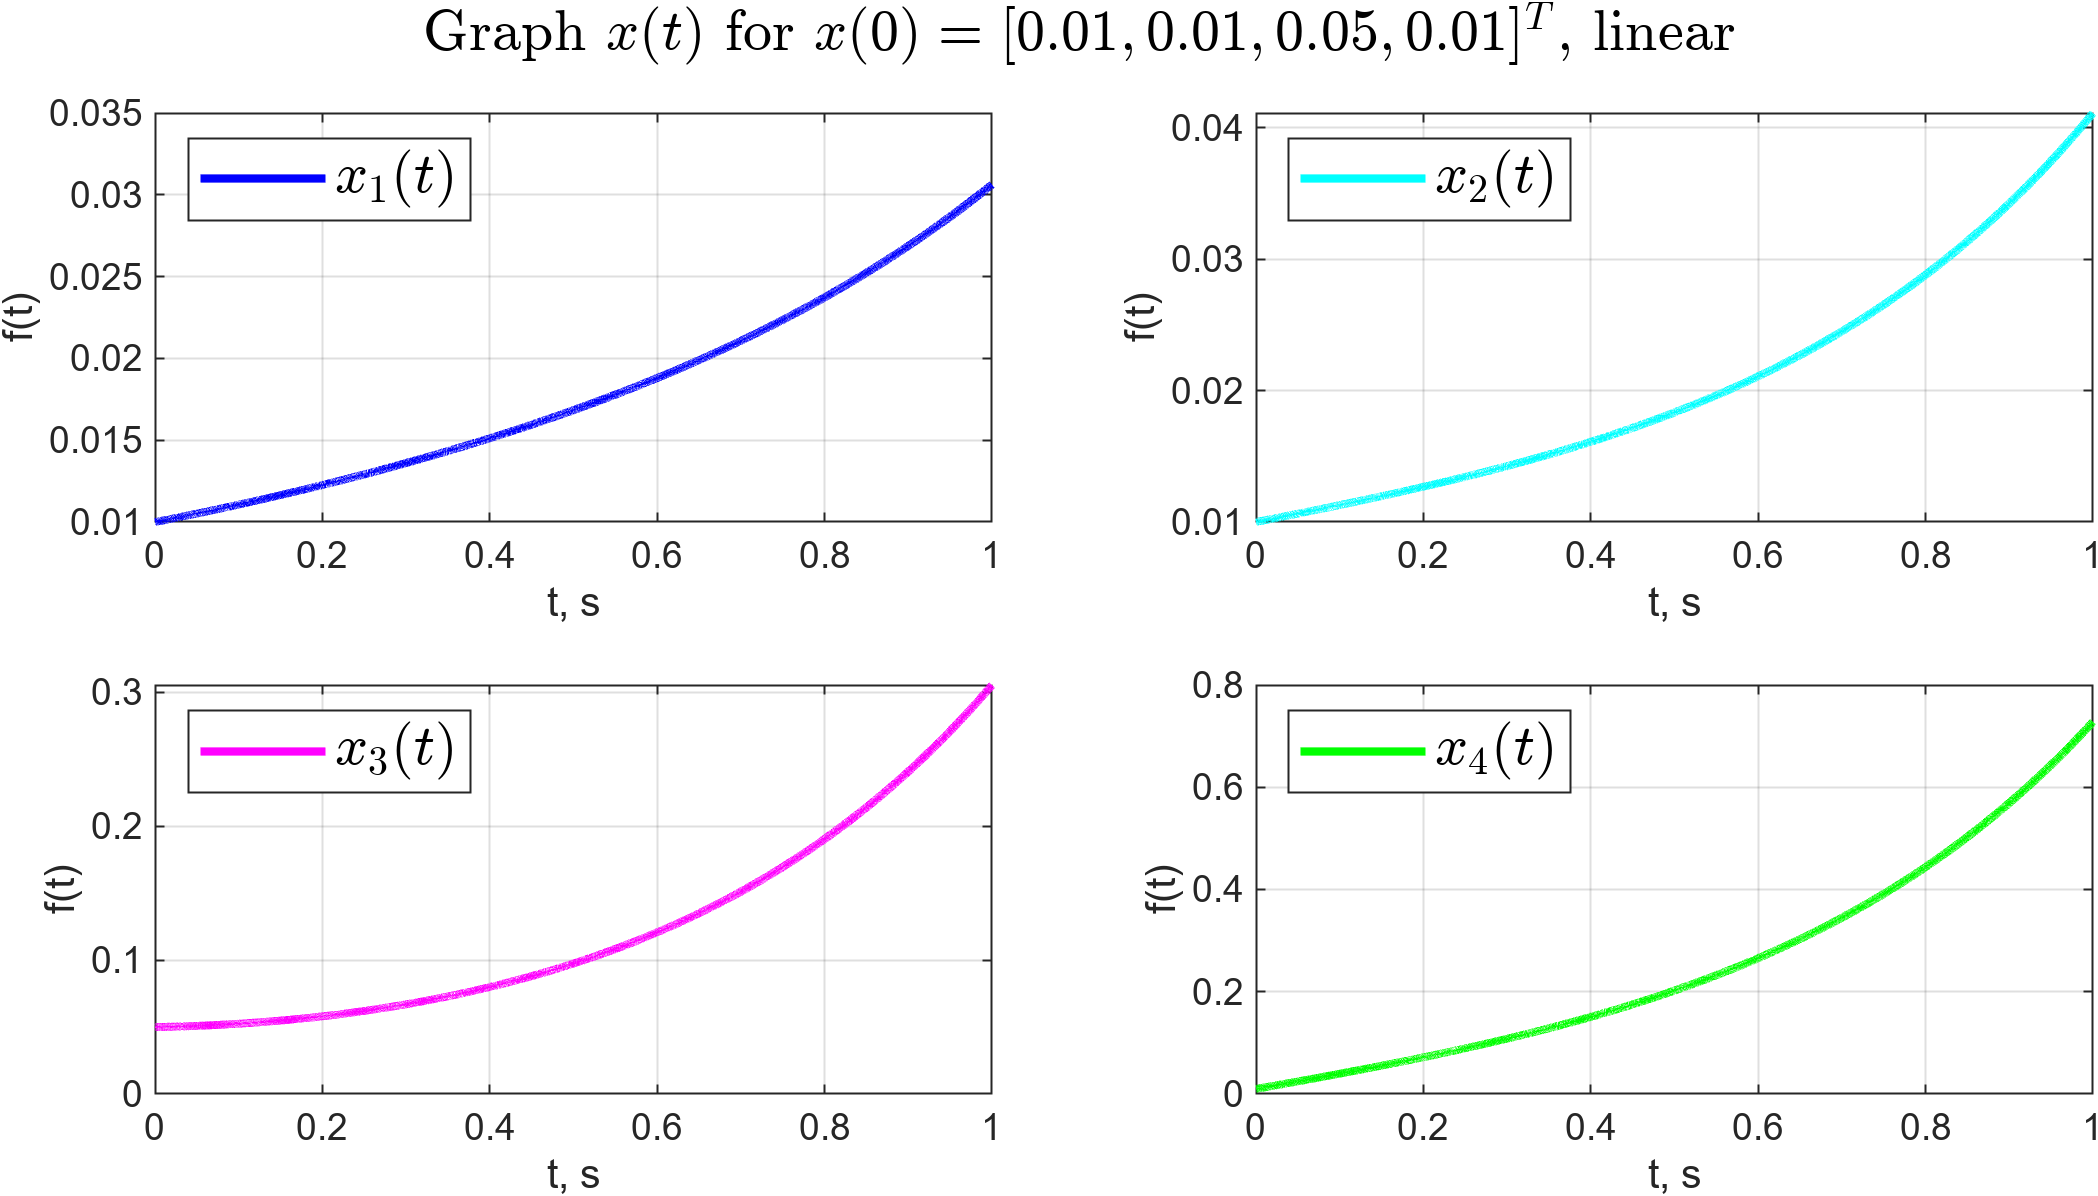
\includegraphics[width=1\linewidth]{pic/2_x_lin_02_sm.png}}
\caption{График вектора состояния линеаризованной системы, время моделирования $t=1$ с, начальные условия $x_{0_2}$.}
\label{2_x_lin_02_sm}
\end{figure}

\begin{figure}[!h]
\center{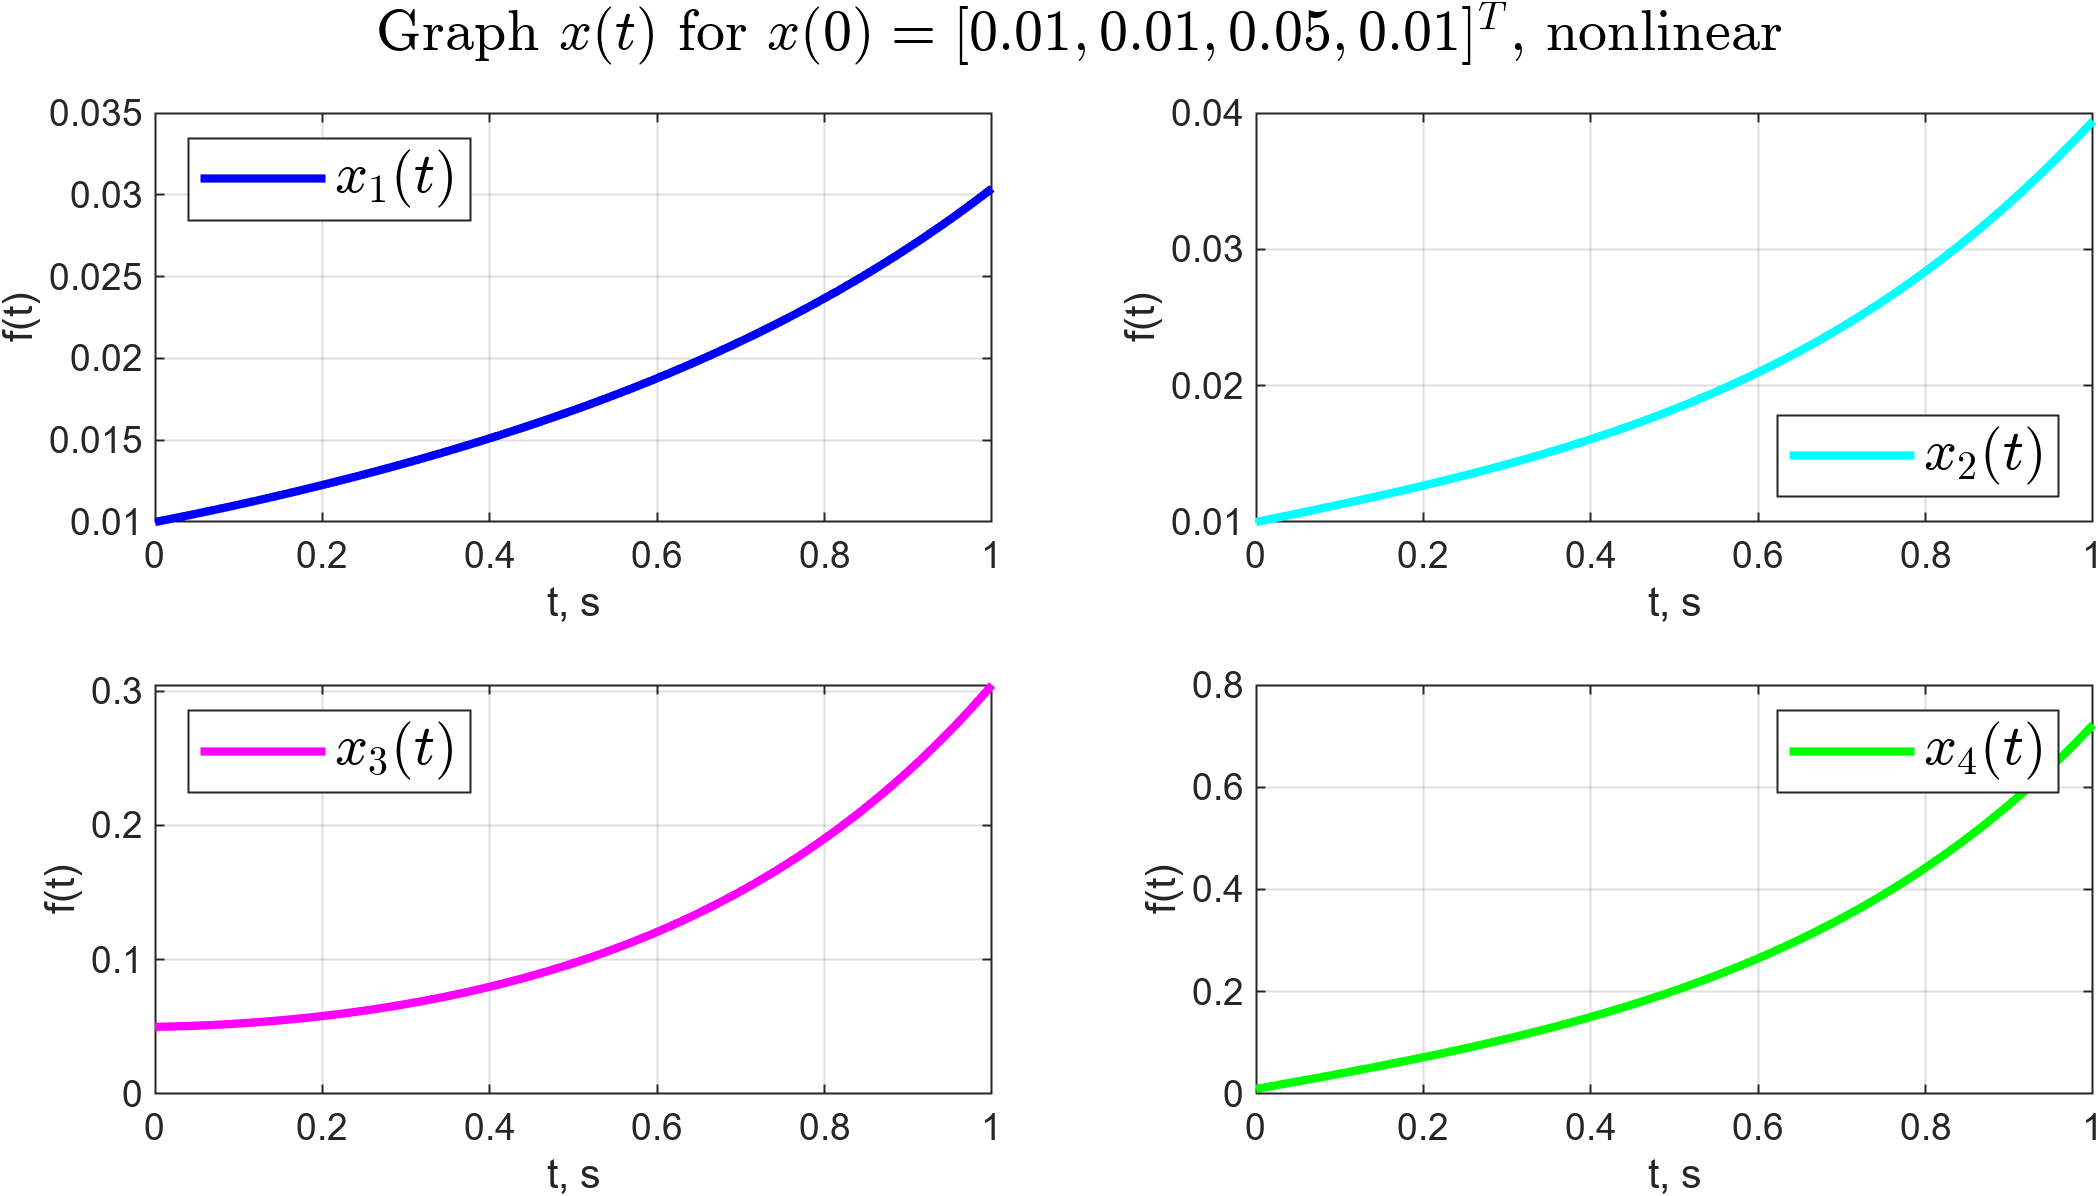
\includegraphics[width=1\linewidth]{pic/2_x_nlin_02_sm.png}}
\caption{График вектора состояния исходной системы, время моделирования $t=1$ с, начальные условия $x_{0_2}$.}
\label{2_x_nlin_02_sm}
\end{figure}

\begin{figure}[!h]
\center{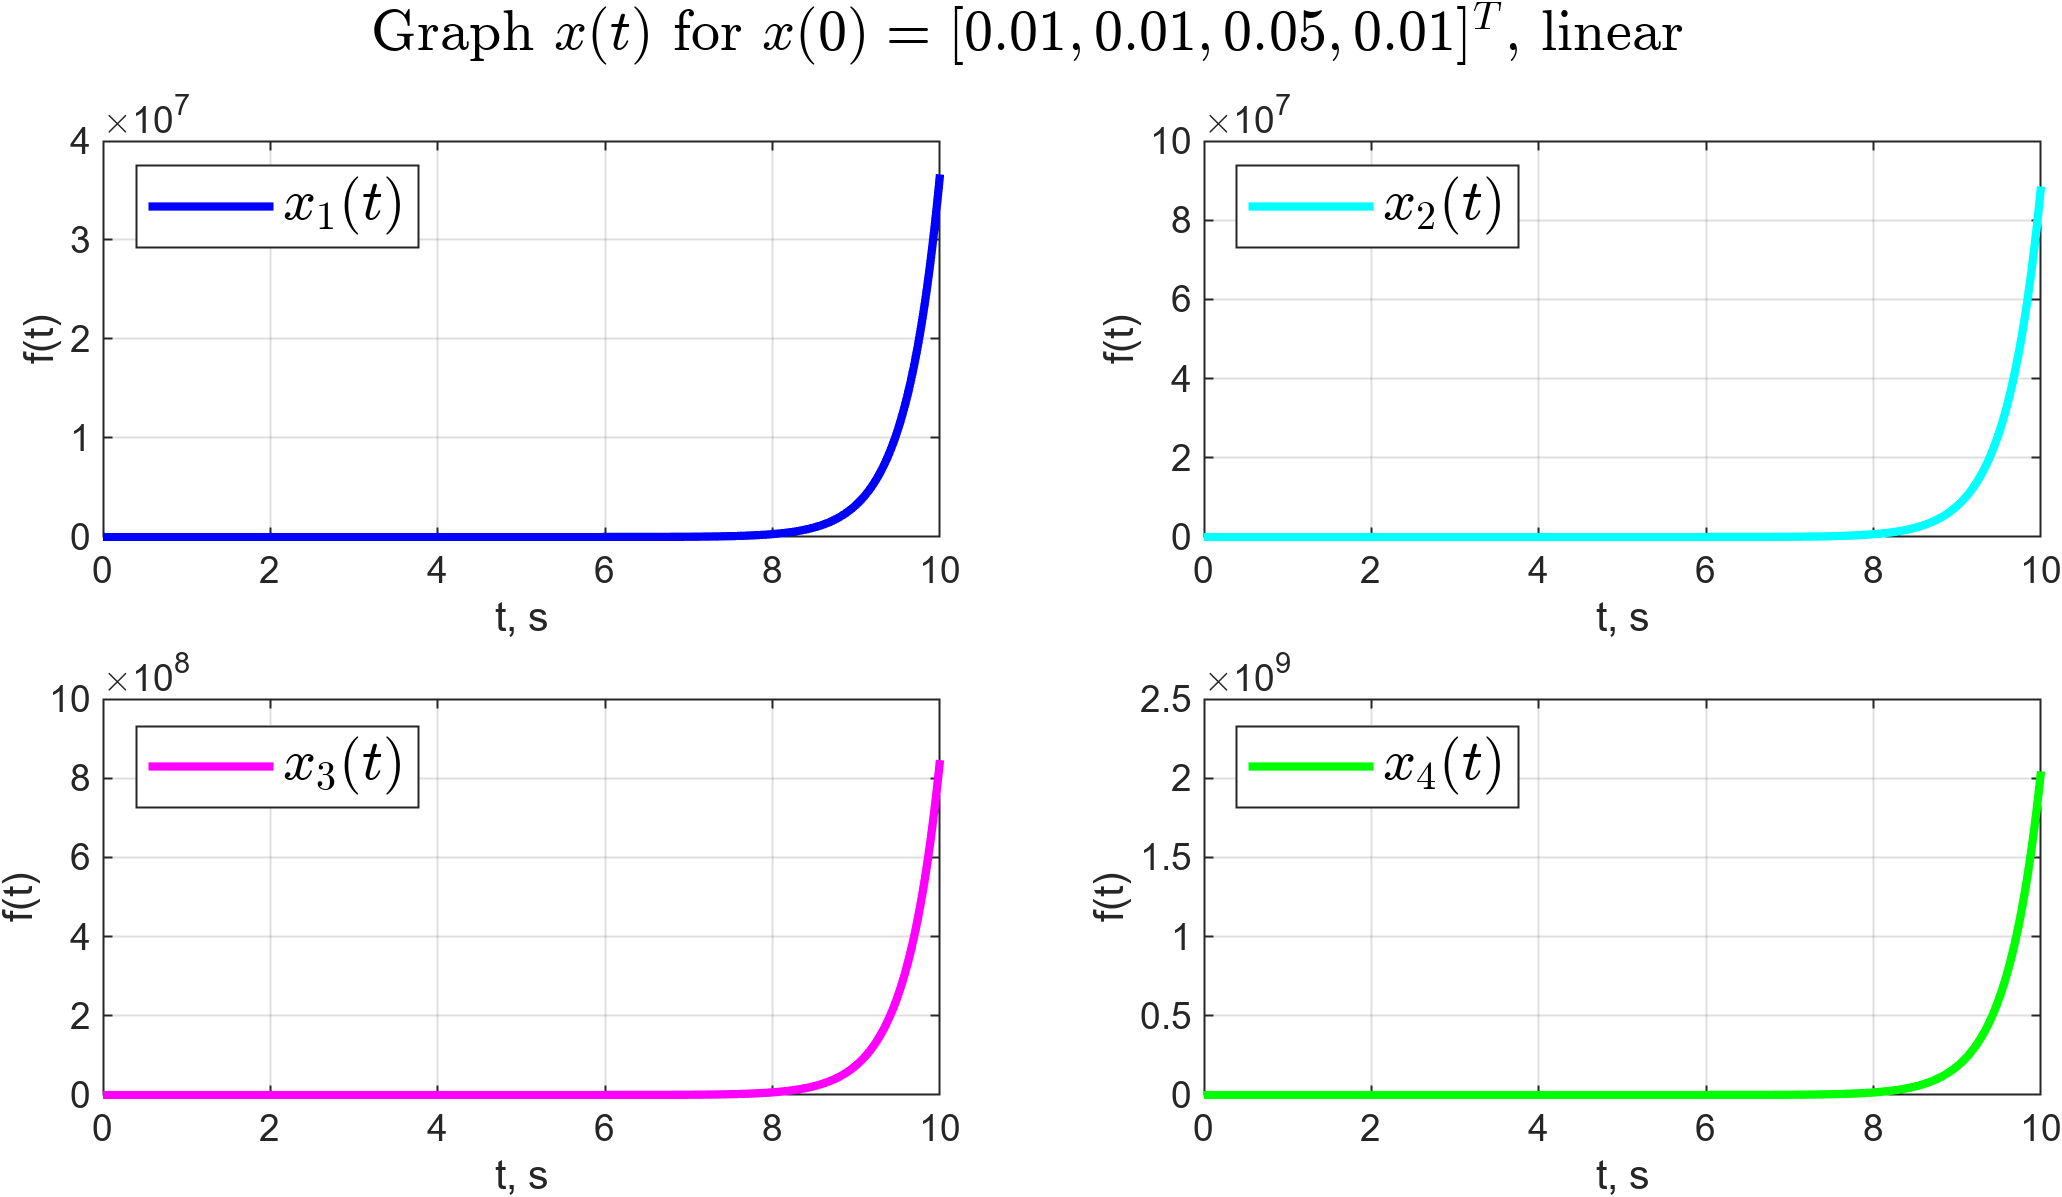
\includegraphics[width=1\linewidth]{pic/2_x_lin_02_lg.png}}
\caption{График вектора состояния линеаризованной системы, время моделирования $t=10$ с, начальные условия $x_{0_2}$.}
\label{2_x_lin_02_lg}
\end{figure}

\begin{figure}[!h]
\center{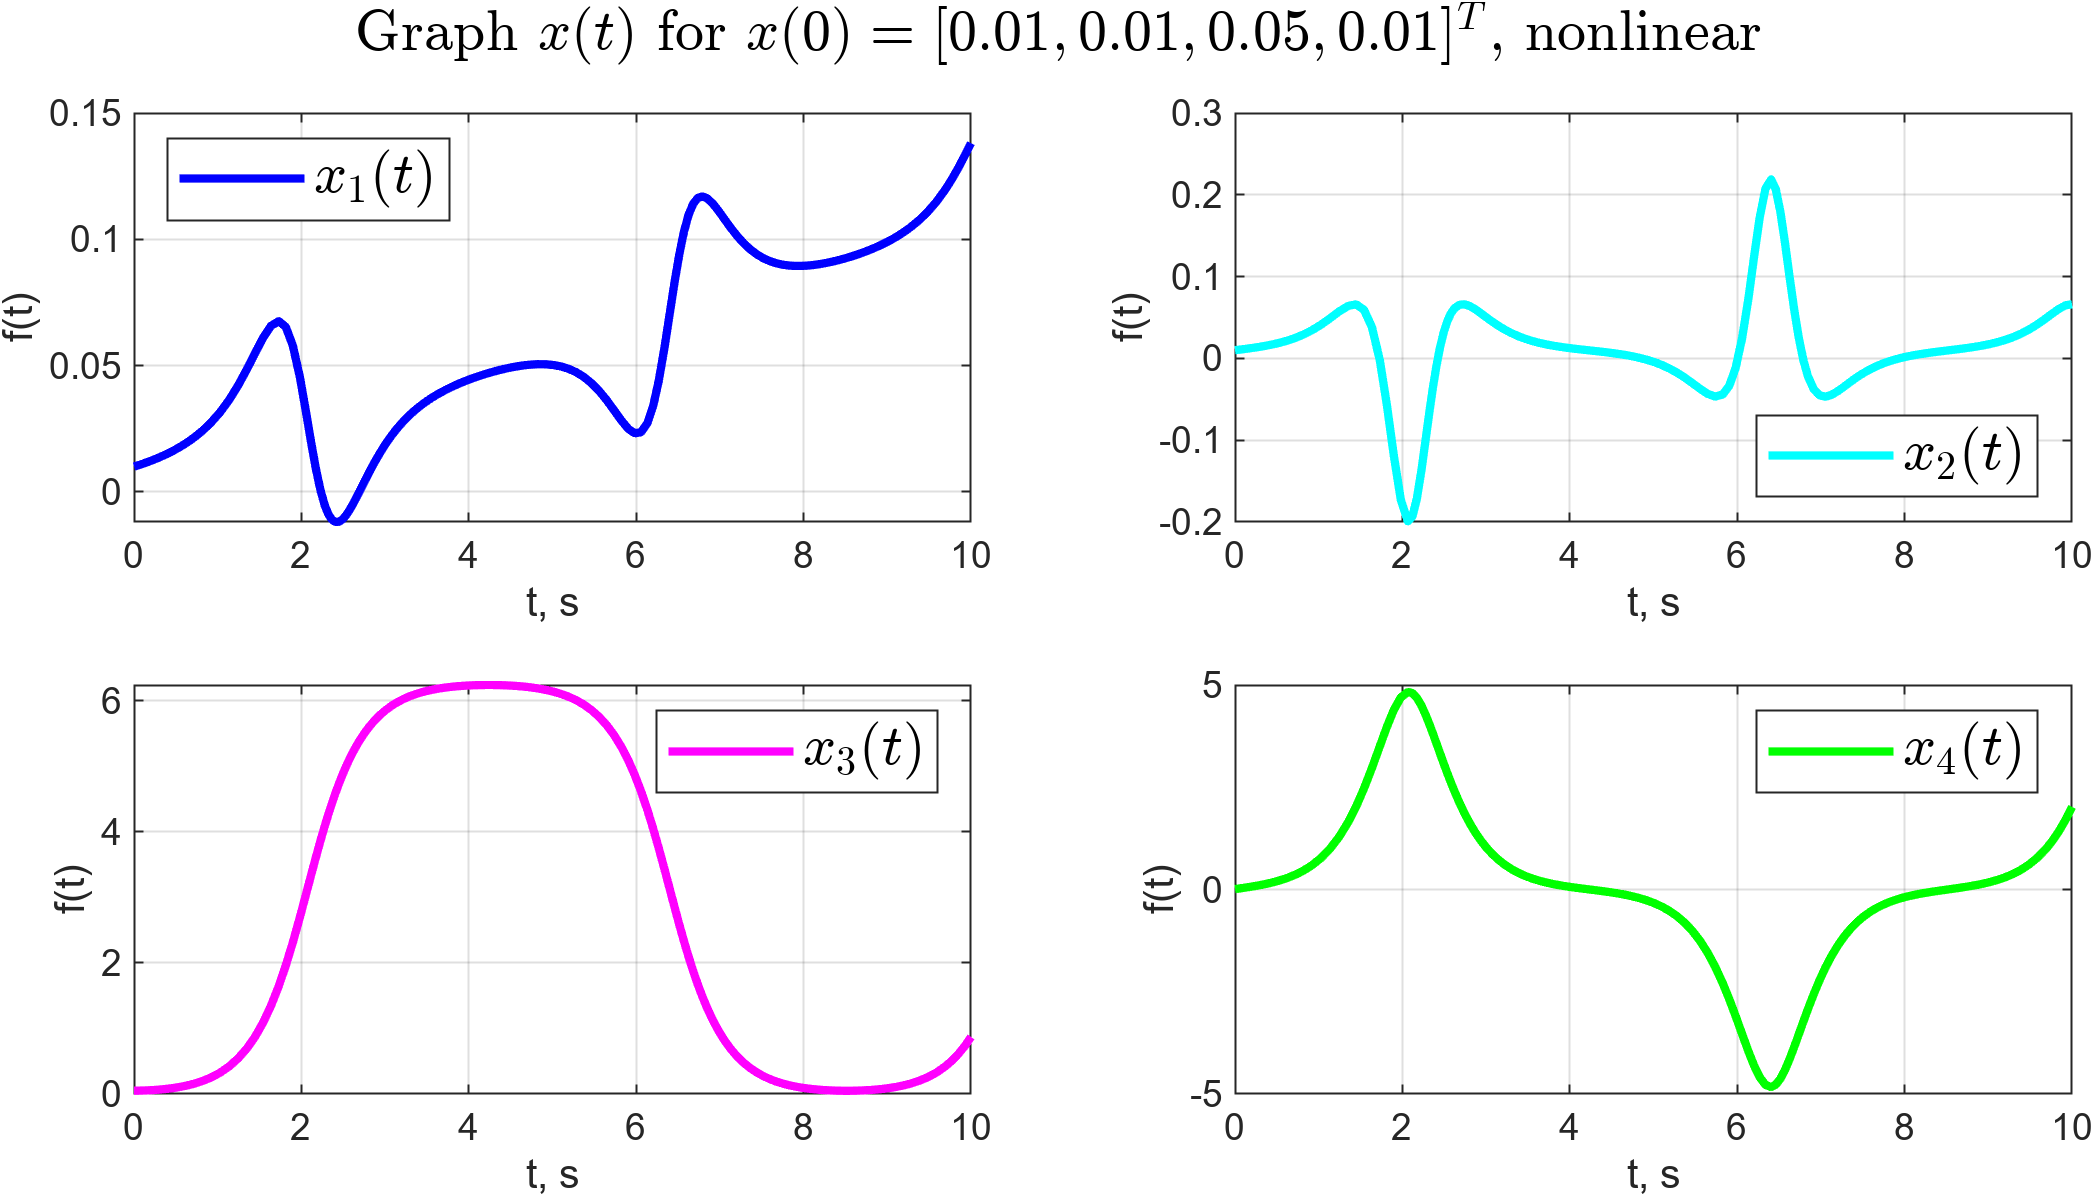
\includegraphics[width=1\linewidth]{pic/2_x_nlin_02_lg.png}}
\caption{График вектора состояния исходной системы, время моделирования $t=10$ с, начальные условия $x_{0_2}$.}
\label{2_x_nlin_02_lg}
\end{figure}




\newpage
\,
\newpage



Заметим, что поведение линеаризованной и исходной системы вновь схожи при малом времени моделирования $t=1$ c (рисунки \ref{2_x_lin_02_sm} и \ref{2_x_nlin_02_sm}). При увеличении времени моделирования до $t=10$ с линеаризованная система вновь сильно отличается от исходной. Кроме того, теперь маятник совершает колебания от $\varphi \approx 0$ до $\varphi \approx 2 \pi$. 




Далее рассмотрим поведение системы при начальных условиях $x_{0_3}$ -- здесь значения также близки к нулю, но теперь больше начальная скорость тележки $x_2(0)$.

\begin{figure}[!h]
\center{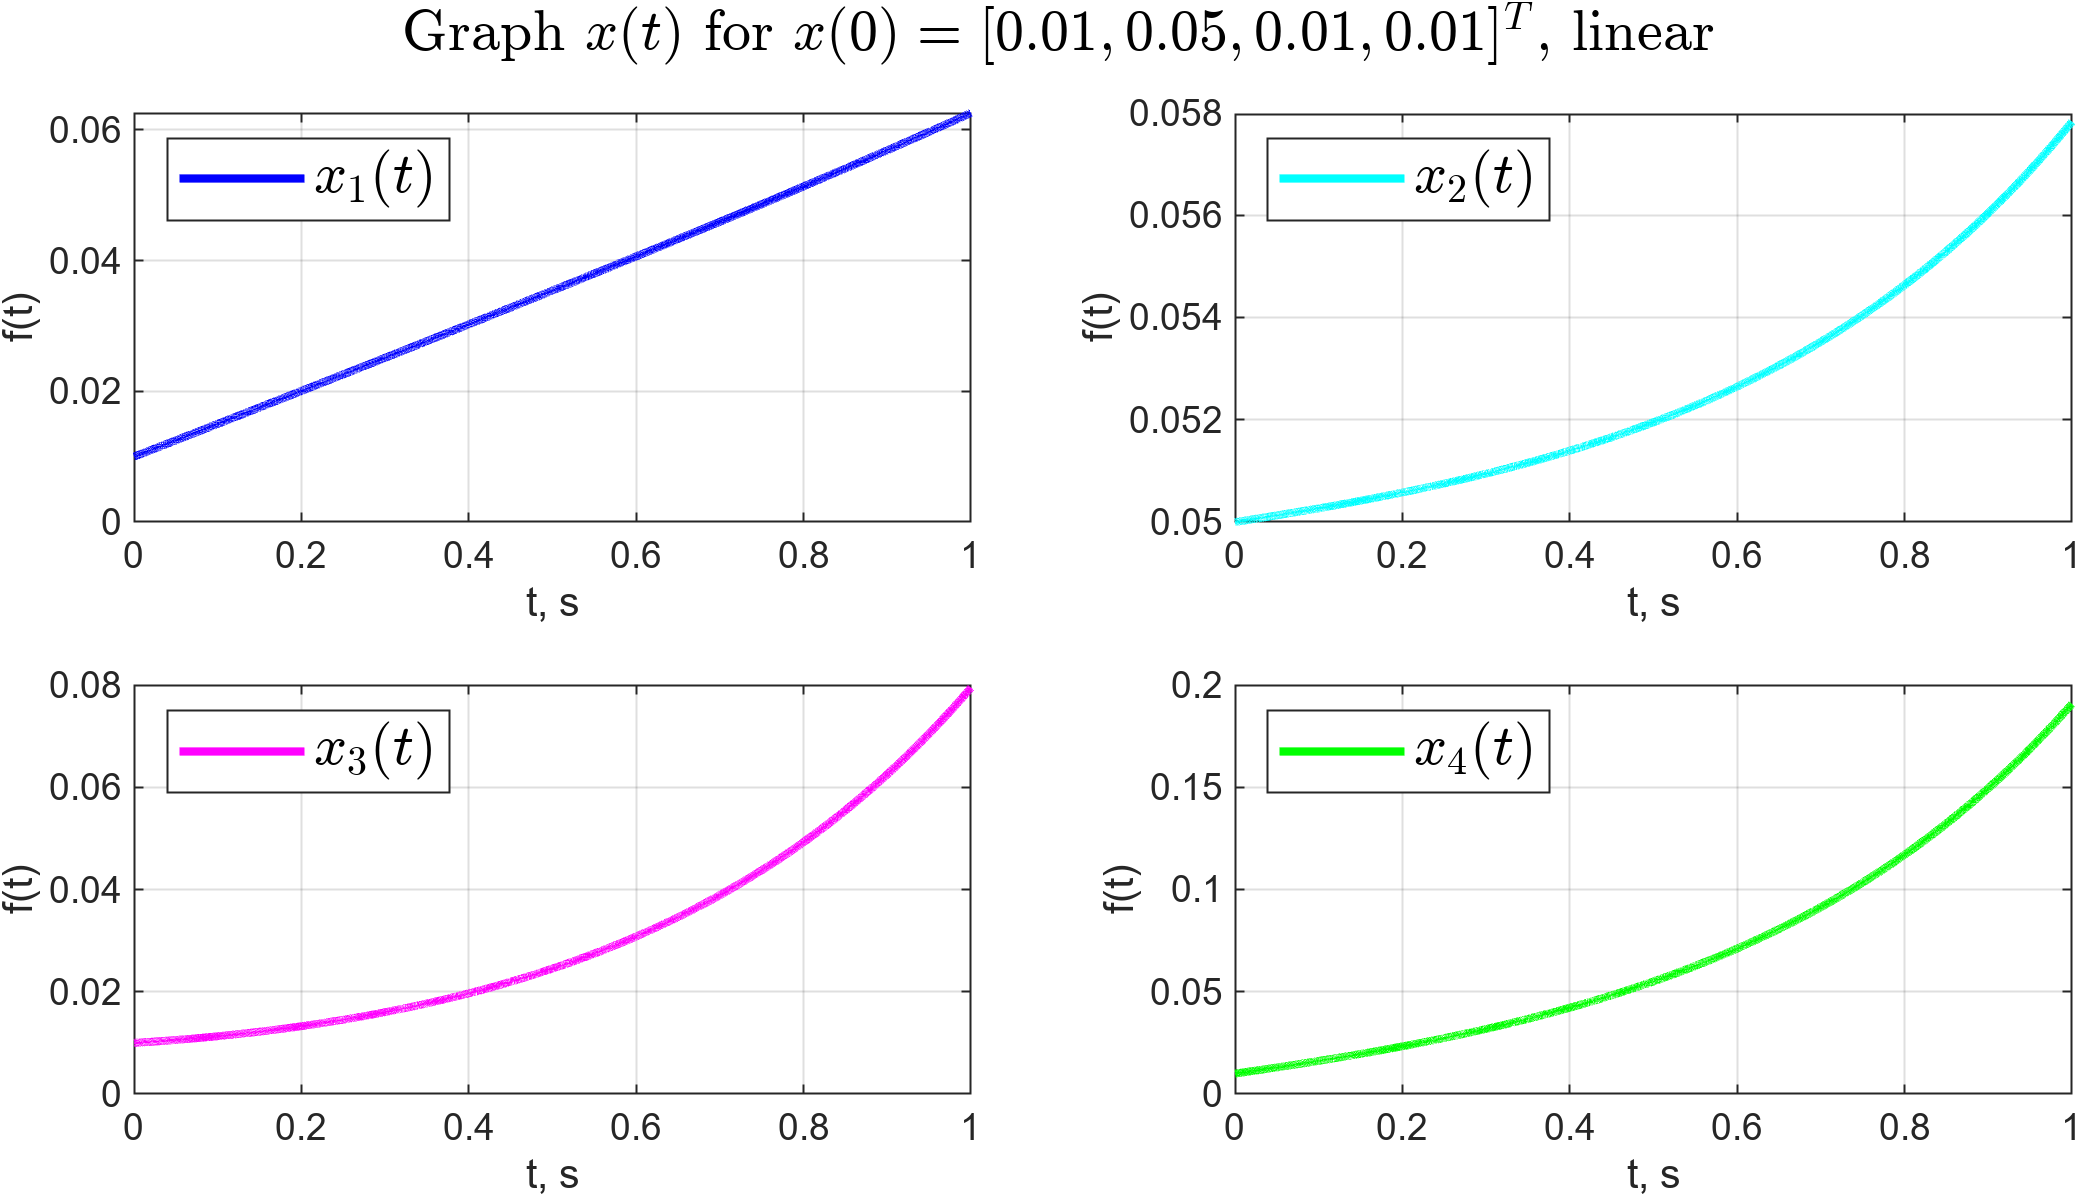
\includegraphics[width=1\linewidth]{pic/2_x_lin_03_sm.png}}
\caption{График вектора состояния линеаризованной системы, время моделирования $t=1$ с, начальные условия $x_{0_3}$.}
\label{2_x_lin_03_sm}
\end{figure}

\begin{figure}[!h]
\center{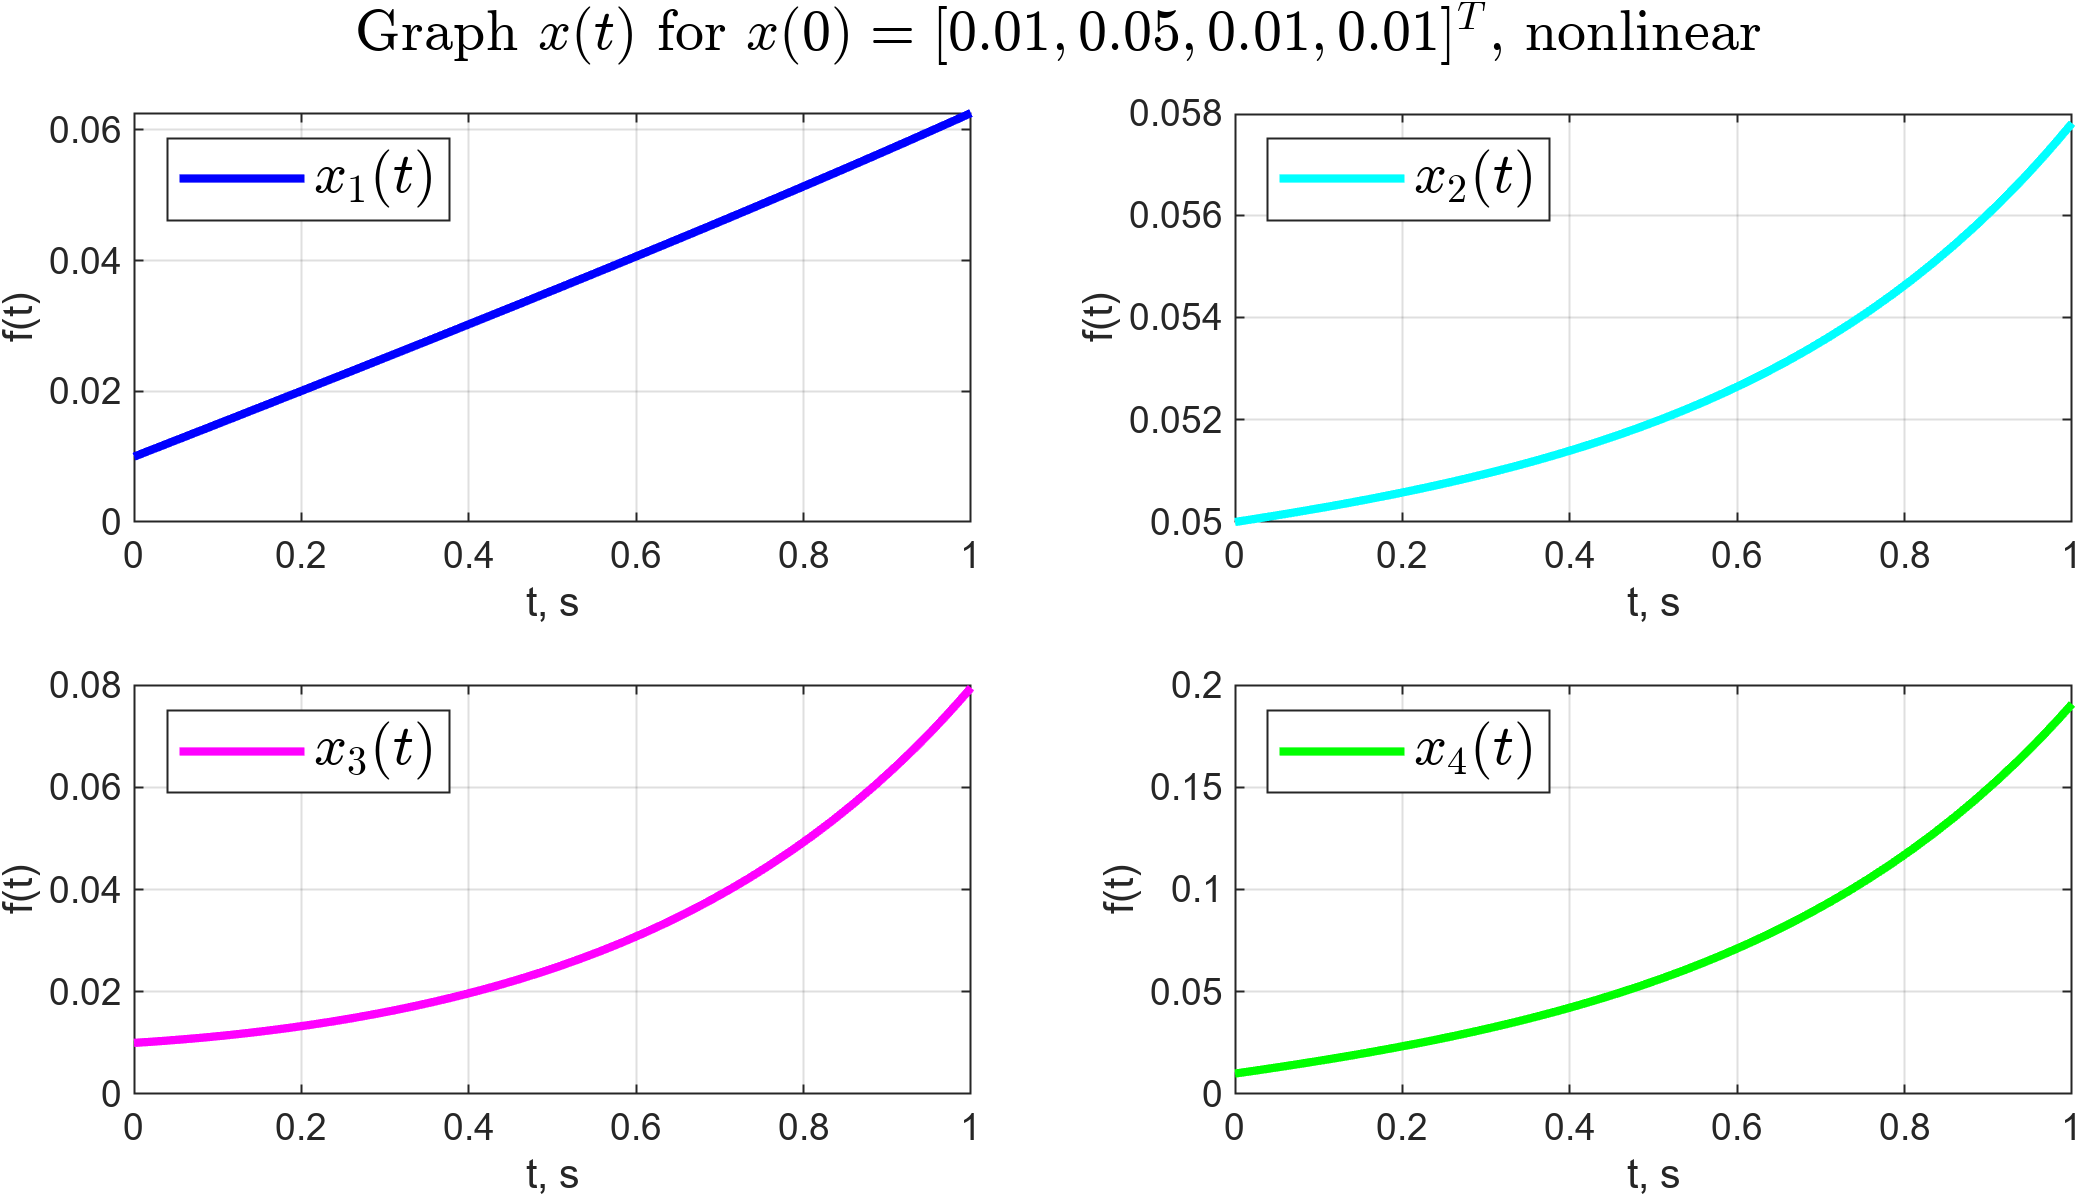
\includegraphics[width=1\linewidth]{pic/2_x_nlin_03_sm.png}}
\caption{График вектора состояния исходной системы, время моделирования $t=1$ с, начальные условия $x_{0_3}$.}
\label{2_x_nlin_03_sm}
\end{figure}

\begin{figure}[!h]
\center{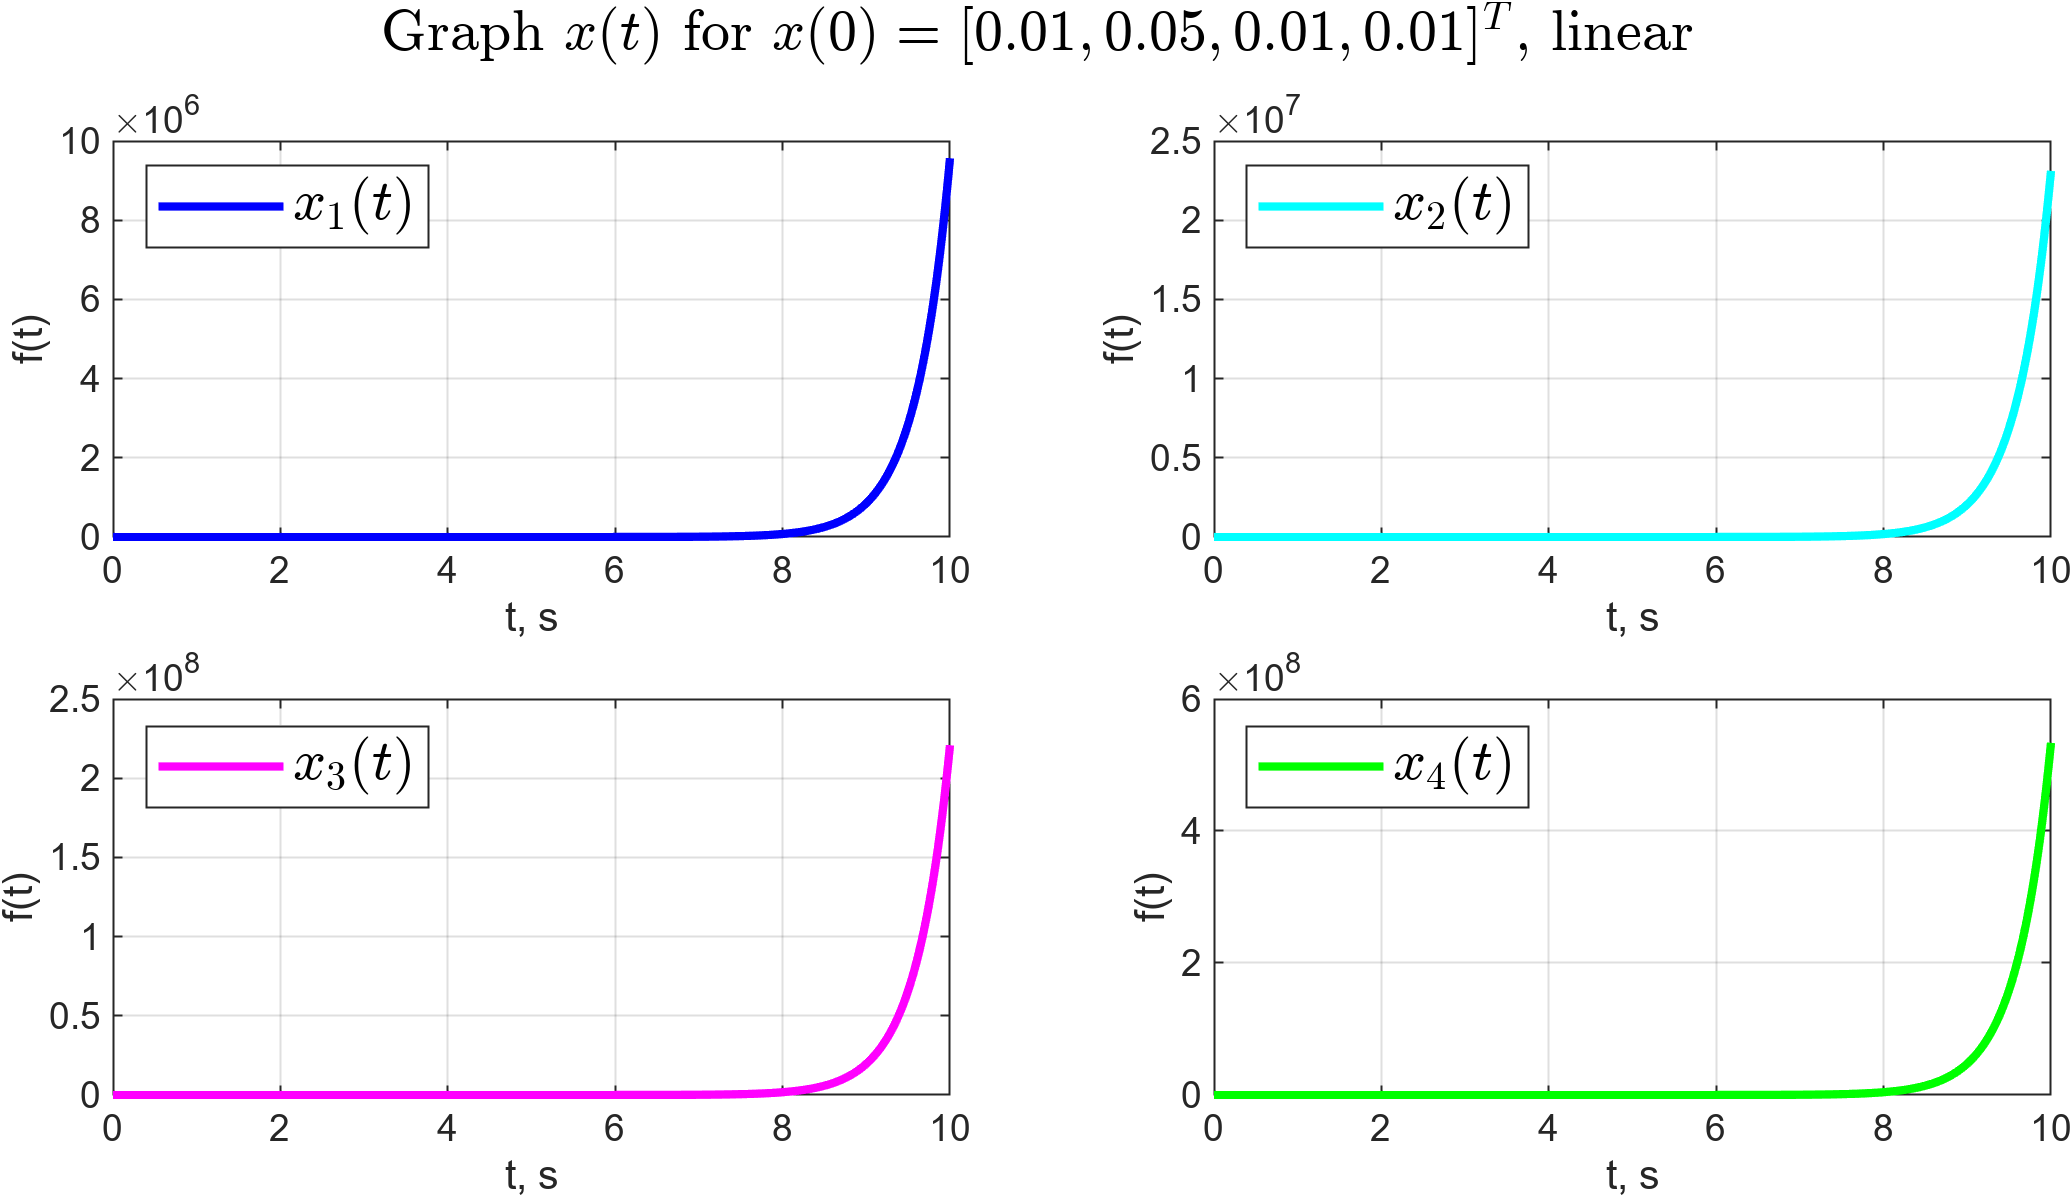
\includegraphics[width=1\linewidth]{pic/2_x_lin_03_lg.png}}
\caption{График вектора состояния линеаризованной системы, время моделирования $t=10$ с, начальные условия $x_{0_3}$.}
\label{2_x_lin_03_lg}
\end{figure}

\begin{figure}[!h]
\center{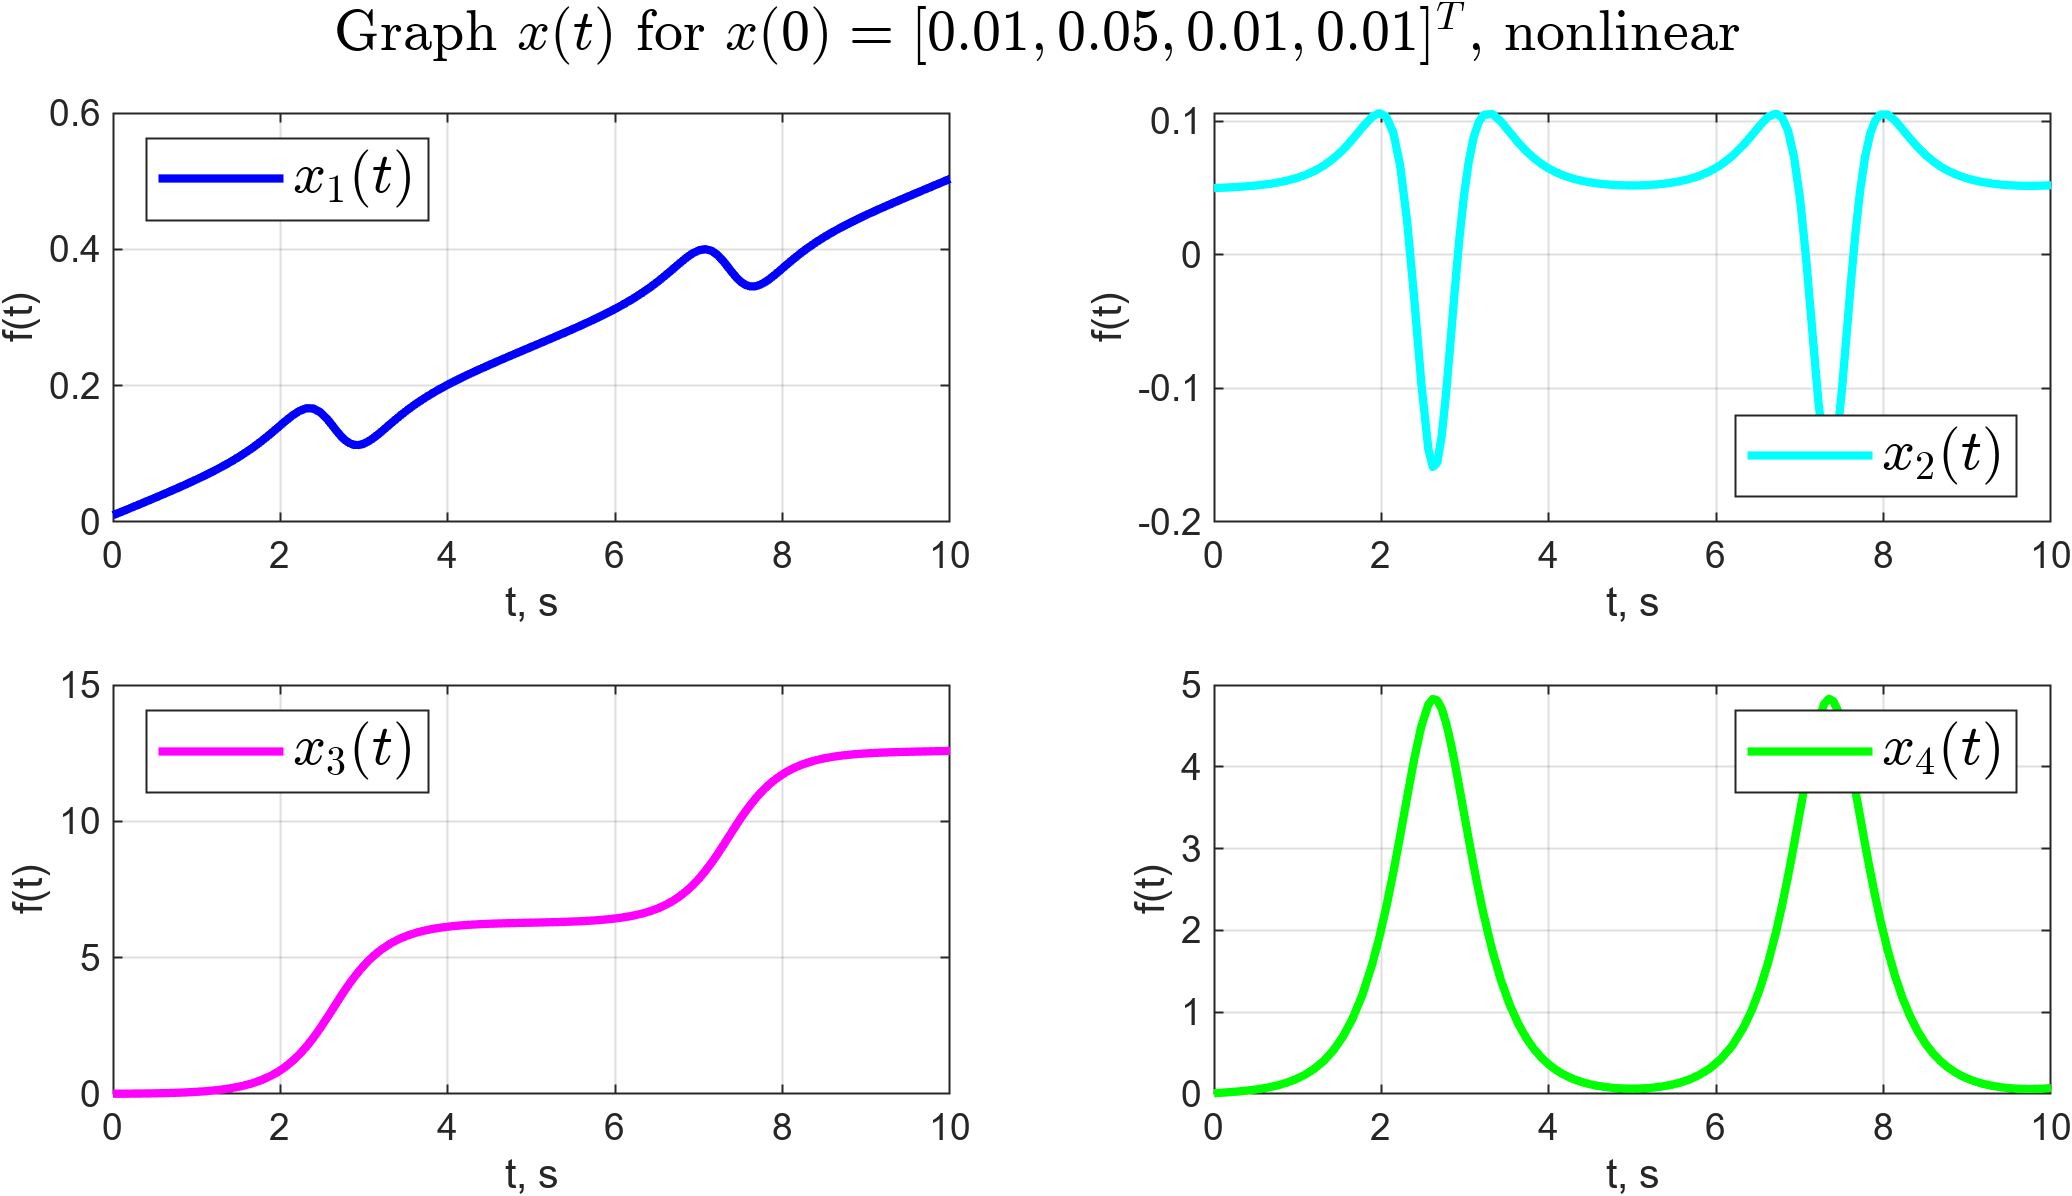
\includegraphics[width=1\linewidth]{pic/2_x_nlin_03_lg.png}}
\caption{График вектора состояния исходной системы, время моделирования $t=10$ с, начальные условия $x_{0_3}$.}
\label{2_x_nlin_03_lg}
\end{figure}
\newpage
\,
\newpage
 Для малого времени моделирования поведение линеаризованной и исходной систем вновь схожи, кроме того, заметим более быстрой рост координаты тележки, чем в предыдущих случаях. На небольшом промежутки времени также наблюдается траектория близкая к линейной, что не характерно для ранее рассмотренных начальных условий.
\endinput